\chapter{相关文献综述}

随着智慧交通系统的不断发展,多目标跟踪技术在交通流量监测、智能驾驶辅助、交通事件预警等方面发挥着越来越重要的作用。本节综述了多目标跟踪技术的发展历程、在智慧交通系统中的应用,以及现有算法的优缺点,旨在为面向智慧交通场景的多目标跟踪算法研究提供理论基础和研究方向\cite{Geiger2012CVPR}。

\section{多目标跟踪技术发展历程}

\subsection{早期的多目标跟踪方法}

多目标跟踪技术的发展可以追溯到20世纪60年代,当时主要应用于军事领域,如雷达目标跟踪。早期的方法主要基于卡尔曼滤波(Kalman Filter)和联合概率数据关联(JPDA)算法。卡尔曼滤波是一种基于线性动态系统的递归滤波算法,能够对目标的状态进行估计和预测,但对非线性系统的适应性较差。JPDA算法通过计算目标与观测数据之间的关联概率,解决多目标跟踪中的数据关联问题,但在目标密集或遮挡严重的情况下,跟踪性能会显著下降\cite{milan2016mot16}。

\subsection{基于数据关联的多目标跟踪方法法}

随着计算机视觉技术的发展,基于数据关联的多目标跟踪方法逐渐兴起。这些方法通常将目标检测和数据关联分开处理。首先,使用目标检测算法(如背景差分法、光流法等)提取每一帧图像中的目标候选区域,然后通过数据关联算法(如匈牙利算法、贪婪算法等)将目标候选与已有的轨迹进行匹配,从而实现多目标跟踪。这类方法的优点是实现相对简单,能够处理一定数量的目标。然而,当目标数量较多、遮挡频繁或目标外观相似时,数据关联的准确性和效率会受到很大影响\cite{马昌庆 2021 面向大场景监控视频的行人多目标跟踪算法研究}。

\subsection{基于深度学习的多目标跟踪方法}

近年来,深度学习技术的快速发展为多目标跟踪带来了新的机遇。基于深度学习的多目标跟踪方法主要分为两类:一类是基于检测的跟踪(Track-by-Detection),另一类是端到端的跟踪(End-to-End Tracking)。\cite{黄晓舸 2024 有向无环图区块链辅助深度强化学习的智能驾驶策略优化算法}基于检测的跟踪方法首先使用深度学习目标检测算法(如YOLO、Faster R-CNN等)检测每一帧图像中的目标,然后通过数据关联算法将检测结果与已有轨迹进行匹配。这些方法能够充分利用深度学习模型的强大特征提取能力,提高目标检测的准确性和鲁棒性,从而提升跟踪性能。然而,数据关联仍然是一个挑战,特别是在复杂场景下。端到端的跟踪方法则尝试将目标检测和数据关联整合到一个深度学习模型中,直接从输入图像序列中输出目标轨迹。这类方法的优点是能够自动学习目标的外观和运动特征,避免了复杂的预处理和后处理步骤,但目前仍处于发展阶段,存在模型复杂度高、训练难度大等问题\cite{胡玉杰 2021 面向复杂场景的多目标跟踪算法研究}。

\begin{figure}[htbp] % 可以是h(here),t(top),b(bottom),p(page of floats)
	\centering
	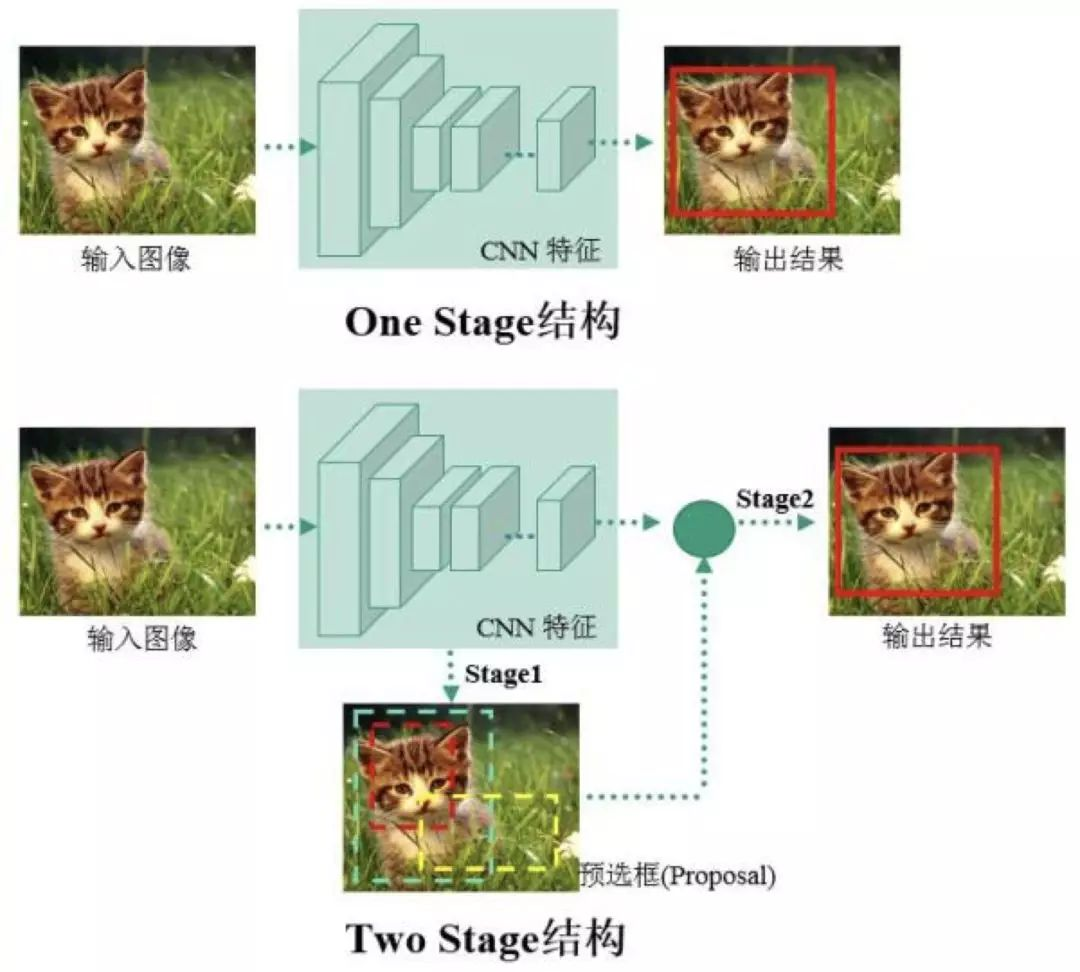
\includegraphics[width=1\textwidth]{p1} % 假设图片文件名为car.pdf或car.png等,位于当前工作目录
	\caption{深度学习} % 图片标题
	\label{fig:p1} % 用于引用的标签
\end{figure}

\section{智慧交通系统中的多目标跟踪应用}

应用包括但不限于交通流量监测、智能驾驶辅助和交通事件预警。

\subsection{交通流量监测}
在智慧交通系统中,多目标跟踪技术可用于实时监测道路上的车辆流量、车速分布、车道占用率等交通参数。通过在关键路口或路段安装摄像头,利用多目标跟踪算法对车辆进行跟踪,可以准确统计车辆的数量、行驶方向和速度,为交通管理部门提供实时的交通信息,以便及时调整交通信号控制策略、疏导交通拥堵。例如,在城市交通繁忙的路口,多目标跟踪系统可以实时监测车辆的排队长度和通行情况,为智能交通信号灯控制系统提供数据支持,优化信号灯的时长分配,提高路口的通行效率\cite{付裕 2023 单源摄像头下的行人多目标跟踪研究}。


\begin{figure}[htbp] % 可以是h(here),t(top),b(bottom),p(page of floats)
	\centering
	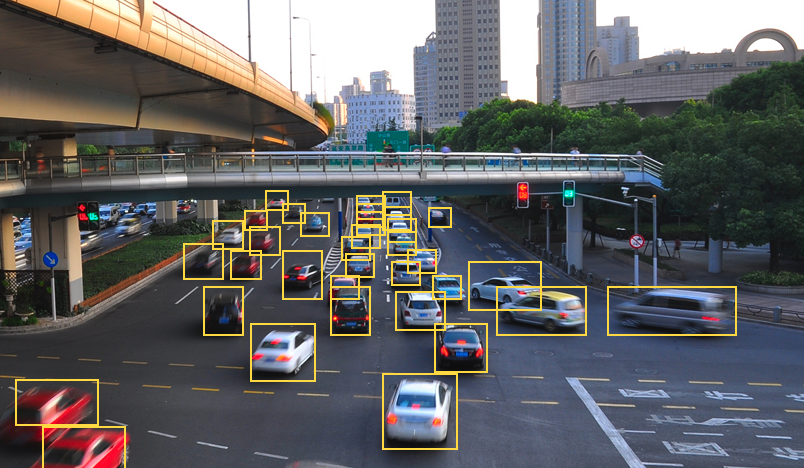
\includegraphics[width=1\textwidth]{p2} % 假设图片文件名为car.pdf或car.png等,位于当前工作目录
	\caption{流量监测} % 图片标题
	\label{fig:p2} % 用于引用的标签
\end{figure}


\subsection{智能驾驶辅助}
多目标跟踪技术在智能驾驶辅助系统中也具有重要应用。自动驾驶车辆需要实时感知周围环境中的其他车辆、行人和障碍物的位置和运动状态,以做出安全的驾驶决策。多目标跟踪算法可以结合车辆的传感器数据(如摄像头、激光雷达、毫米波雷达等),对周围目标进行准确跟踪,为自动驾驶车辆提供可靠的环境感知信息。例如,通过多目标跟踪算法,自动驾驶车辆可以提前预测前方车辆的行驶意图,及时调整车速和行驶路线,避免碰撞事故的发生。此外,多目标跟踪技术还可以用于车道偏离预警、前车碰撞预警等功能,提高驾驶的安全性和舒适性\cite{王宇唯 2023 基于CARLA的仿真数据集生成框架研究}。



\begin{figure}[htbp] % 可以是h(here),t(top),b(bottom),p(page of floats)
	\centering
	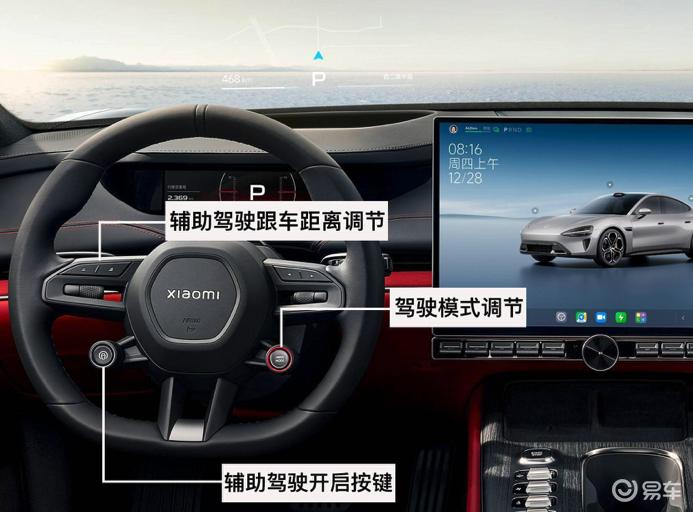
\includegraphics[width=1\textwidth]{p3} % 假设图片文件名为car.pdf或car.png等,位于当前工作目录
	\caption{辅助驾驶} % 图片标题
	\label{fig:p3} % 用于引用的标签
\end{figure}



\subsection{交通事件预警}
多目标跟踪技术还可以用于交通事件的预警和检测。通过对道路上目标的跟踪和分析,可以实时发现异常的交通行为,如车辆逆行、违规变道、行人闯红灯等,及时发出预警信息,提醒交通管理部门和驾驶员采取相应的措施。例如,在高速公路场景中,多目标跟踪系统可以实时监测车辆的行驶轨迹,当发现有车辆偏离正常行驶路线时,及时发出车道偏离预警,提醒驾驶员注意行驶安全。在城市路口,多目标跟踪系统可以检测行人和车辆的冲突情况,为交通信号灯控制系统提供预警信息,提前调整信号灯状态,避免交通事故的发生\cite{zhang2021survey}。




\begin{figure}[htbp] % 可以是h(here),t(top),b(bottom),p(page of floats)
	\centering
	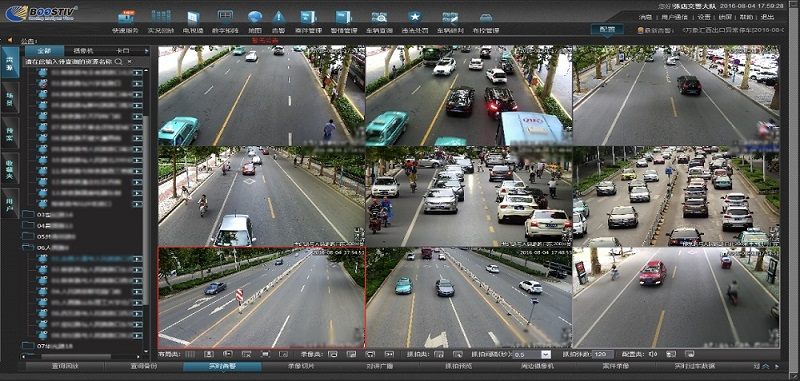
\includegraphics[width=1\textwidth]{p4} % 假设图片文件名为car.pdf或car.png等,位于当前工作目录
	\caption{交通事件预警} % 图片标题
	\label{fig:p4} % 用于引用的标签
\end{figure}




\section{现在多目标跟踪算法的优缺点分析}

\subsection{优点}
目标检测精度高:借助深度学习目标检测算法,能够准确地检测出每一帧图像中的目标,为后续的跟踪提供可靠的基础。

灵活性强:可以方便地与其他技术(如数据关联算法、外观特征提取算法等)结合,以适应不同的应用场景和需求。

可扩展性好:在目标检测部分,可以通过调整深度学习模型的结构和参数,提高对不同类型目标的检测能力,从而扩展跟踪算法的应用范围\cite{tang2021multiple}。
\subsection{缺点}
数据关联复杂:当目标数量较多、遮挡频繁或目标外观相似时,数据关联的准确性和效率会受到很大影响,容易出现轨迹断裂或错误关联的情况。

计算复杂度高:目标检测和数据关联通常需要分别进行,计算复杂度较高,特别是在实时性要求较高的场景下,可能难以满足实时跟踪的要求。

对目标外观变化敏感:如果目标在跟踪过程中发生较大的外观变化(如车辆的遮挡、行人的姿态变化等),基于外观特征的匹配可能会失效,导致跟踪失败\cite{sun2020sparse}。
















